\documentclass[12pt,phd,times]{pkmthesis}
\usepackage{amsmath,epsfig,graphicx,setspace,url,float}
\usepackage{pstricks,colortab,pifont}
\usepackage{lscape,multicol,multirow,longtable,subfigure}
\usepackage{cite,bm}
\usepackage[english]{babel}
\usepackage[small,bf]{caption}
\captionsetup[table]{position=top}
\setlength{\textfloatsep}{1cm}
\setlength{\abovecaptionskip}{8pt}
\setlength{\belowcaptionskip}{8pt}
\usepackage{array,tabularx}
\usepackage{tikz}
\usetikzlibrary{arrows.meta,positioning}
\tikzset{every picture/.append style={execute at begin picture={\linespread{1}\selectfont}}}
\newcolumntype{Y}{>{\raggedright\arraybackslash}X}
\usepackage{hyperref}
\usepackage{extra_functions}
\normalem
%*************************************************  MARGINS  ************************************************
\hoffset 0in
\voffset 0in
%\oddsidemargin 0.40cm
\oddsidemargin -0cm
\evensidemargin -0cm
\marginparsep 0in
\topmargin -0.25cm
\textwidth 16cm
\textheight 23.5cm
\footskip 1.5cm

%*************************************************************************************************************

\usepackage{fancyhdr}
\pagestyle{fancy}

%*************************************************************************************************************

\renewcommand{\chaptermark}[1]{\markboth{\thechapter.\ #1}{}}
\renewcommand{\sectionmark}[1]{\markright{\thesection\ #1}}

%\fancyhf{} \fancyhead[LE]{\bfseries\nouppercase{\leftmark}}
%\fancyhead[RO]{\bfseries\nouppercase{\rightmark}}

%*************************************************************************************************************
% HEADER & FOOTER HEADINGS  %PKM 04/07/08
%*************************************************************************************************************

\renewcommand{\headrulewidth}{0.5pt}
\renewcommand{\footrulewidth}{0.5pt}
\addtolength{\headheight}{2pt} % make space for the rule

%*************************************************************************************************************

\fancypagestyle{plain}{%
   \fancyhead{} % get rid of headers
   \renewcommand{\headrulewidth}{0pt} % and the line
   \renewcommand{\footrulewidth}{0pt}
}

%*************************************************************************************************************

\fancypagestyle{blank}{%
   \fancyhf{} % get rid of headers and footers
   \renewcommand{\headrulewidth}{0pt} % and the line
   \renewcommand{\footrulewidth}{0pt}
}

%*************************************************************************************************************

\fancypagestyle{abstract}{%
   \fancyhead{}
   \renewcommand{\headrulewidth}{0pt}
   \renewcommand{\footrulewidth}{0.5pt}
}

%*************************************************************************************************************

\fancypagestyle{document}{%
	\fancyhf{} \fancyhead[LE]{\bfseries\nouppercase{\leftmark}}
	\fancyhead[RO]{\bfseries\nouppercase{\rightmark}}
	\fancyfoot[LE,RO]{\bfseries\thepage}
	\renewcommand{\headrulewidth}{0.5pt}
	\renewcommand{\footrulewidth}{0.5pt}
	\addtolength{\headheight}{2pt} % make space for the rule
}

%*************************************************************************************************************
% SUBSECTION DEPTH  PKM on 05/07/08

\setcounter{secnumdepth} {5}
\setcounter{tocdepth} {5}
%\renewcommand{\thesubsubsection}{\thesubsection.\Alph{subsubsection}}   % (PKM 10/07/08- To remove Alpha number on subsubsubsection)

%*************************************************************************************************************
%\renewcommand{\subfigtopskip}{0.3 cm}
%\renewcommand{\subfigbottomskip}{0.2 cm}
%\renewcommand{\subfigcapskip}{0.3 cm}
%\renewcommand{\subfigcapmargin}{0.2 cm}

%*************************************************************************************************************
% PAGE SIZE & HYBERLINKS PKM on 05/07/08

\hypersetup{     a4paper=true,
                 bookmarks,
                 bookmarksopen = true,  %false (18/07/08)
                 bookmarksnumbered = true,
                 breaklinks = true,
                 linktocpage,
                 pagebackref,
                 colorlinks = false,   %true (18/07/08)
                 linkcolor = blue,
                 urlcolor  = blue,
                 citecolor = red,
                 anchorcolor = green,
                 hyperindex = true,
                 linktocpage,
                 pagebackref,
                 hyperfigures,
                 pdftitle={SPEECH ENHANCEMENT},
                 pdfauthor={PKM},
                 pdfsubject={FINAL REPORT},
                 pdfcreator={ACROBAT 9 PROFESSIONAL},
                 pdfkeywords={This PDF is created with ACROBAT PROFESSIONAL 9 with PDFVERSION 1.5}}

%*************************************************************************************************************



\graphicspath{{images/}}
\hypersetup{pdftitle={SecGuard: Risk-Adaptive Isolation for Profit-Aware 5G Network Slicing},pdfauthor={Ayush Vishwakarma},pdfsubject={Master's Thesis Project Report}}
\raggedbottom

\begin{document}
\setcounter{page}{1}\pagenumbering{roman}
\doublespacing

\thispagestyle{empty}
\pdfbookmark{Title}{Title}
\begin{center}
{\fontsize{15.8pt}{19pt}\selectfont\bfseries SecGuard: Risk-Adaptive Isolation for Profit-Aware 5G Network Slicing\par}
\vspace*{0.13in}
{\large\bfseries Master's Thesis Project I (MTP-I)\par}
{\large Subject Code: ITIT-5199\par}
\vspace*{0.13in}
{\large\emph{A report submitted in partial fulfilment for the award of the degree of}\par}
{\large\emph{IPG Masters of Technology}\par}
{\large in\par}
{\large Information Technology\par}
{\large By\par}
{\large\bfseries Ayush Vishwakarma : 2022IMT-028\par}
{\large Under the Supervision of\par}
{\large\bfseries Prof. Aditya Trivedi\par}
{\large Department of Information Technology\par}
\end{center}
\begin{figure}[!h]
\centerline{
\includegraphics[width=3cm]{FrontPages/ABVIIITM_logo.jpg}}
\end{figure}
\centerline{\large{ABV-INDIAN INSTITUTE OF INFORMATION TECHNOLOGY}}
\centerline{\large{AND MANAGEMENT GWALIOR}}
\vspace*{0.05in}
\centerline{\large{GWALIOR - 474015, INDIA}}

\clearpage
\thispagestyle{empty}
\pdfbookmark{Declaration}{Declaration}
\begin{center}{\Large\bfseries DECLARATION}\end{center}
\vspace{0.5cm}
\noindent I hereby certify that the work presented in this report, entitled \textbf{SecGuard: Risk-Adaptive Isolation for Profit-Aware 5G Network Slicing}, in partial fulfilment of the requirements for the Integrated Post Graduate M.Tech in Information Technology, is an authentic record of my own work carried out under the supervision of \textbf{Prof. Aditya Trivedi}. Sources of text, figures, and tables taken from other works are cited where applicable.

\vspace{1cm}
\begin{center}
\begin{tabular}{p{0.58\textwidth}p{0.4\textwidth}}
Dated: & \textbf{Signature of the candidate}\\
& \rule{0pt}{1cm}
\end{tabular}
\end{center}
\vspace{1.5cm}
\noindent This is to certify that the above statement made by the candidate is correct to the best of my knowledge.
\vspace{1.5cm}
\begin{center}
\begin{tabular}{p{0.65\textwidth}p{0.3\textwidth}}
Dated: & \textbf{Signature of supervisor}\\
& \rule{0pt}{1cm}
\end{tabular}
\end{center}

\thispagestyle{empty}
\pdfbookmark{Acknowledgements}{Acknowledgements}
\begin{center}{\LARGE\bfseries Acknowledgements}\end{center}
\noindent I am deeply grateful to Prof. Aditya Trivedi for his guidance and mentorship throughout this Master's Thesis Project (MTP). His questions about what a learned method must prove before it is trusted, and his encouragement to test ideas on real equipment rather than in simulation alone, shaped the direction of this work.

I thank the Department of Information Technology for access to the 5G Use Case Lab. I also thank the authors of the base paper for releasing their code publicly, which made the replication reported here possible.

I am grateful to this institution for the opportunity to pursue this MTP and for the resources and facilities it has provided, and to my professors for their mentoring and fair evaluation of my work. Finally, I thank my family and friends for their constant support.

\begin{flushright}\textit{\textbf{Ayush Vishwakarma}}\end{flushright}

\clearpage

\thispagestyle{empty}
\pdfbookmark{Abstract}{Abstract}
\begingroup
\onehalfspacing
\begin{center}\textbf{Abstract}\end{center}
\itshape
\noindent
Network slicing shares radio, transport, and computing resources among services with different performance and isolation needs. The 5Guard allocator models three isolation levels but treats the requested level as fixed. This report presents SecGuard, a risk-adaptive extension that uses traffic-derived threat scores to raise isolation without lowering the tenant's requested service level. A random-forest detector and a threshold policy feed an adapter to the allocation workflow. Admission control and algorithm selection are proposed as later objectives.

In the preliminary synthetic evaluation described in the source report, 30 held-out, trace-derived scenarios were used to compare static 5Guard, fixed SecGuard thresholds, and selected SecGuard thresholds. The selected policy reduced a modeled isolation-exposure proxy by 67.12\% relative to static 5Guard, raised mean profit by 164.9\% relative to fixed thresholds, and retained 90.4\% of static 5Guard mean profit. These results motivate further evaluation; they do not measure attack containment in an operational network.

\medskip\noindent\textbf{Keywords:} 5G network slicing, isolation, threat detection, resource allocation, random forest, security exposure.
\clearpage
\endgroup
\dominitoc\dominilof\dominilot
\fancyhf{}
\fancyhead[LE]{\bfseries\small{\leftmark}}
\fancyhead[RO]{\bfseries\small{\rightmark}}
\fancyfoot[CE,CO]{\bfseries\thepage}
\renewcommand{\baselinestretch}{1}

\pdfbookmark[0]{Contents}{toc}
\fancyhead[LE]{\bfseries\small{Contents}}
\fancyhead[RO]{\bfseries\small{Contents}}
\tableofcontents
\clearpage

\pdfbookmark[1]{List of Figures}{lof}
\addstarredchapter{List of Figures}
\fancyhead[LE]{\bfseries\small{List of Figures}}
\fancyhead[RO]{\bfseries\small{List of Figures}}
\listoffigures
\clearpage

\pdfbookmark[1]{List of Tables}{lot}
\addstarredchapter{List of Tables}
\fancyhead[LE]{\bfseries\small{List of Tables}}
\fancyhead[RO]{\bfseries\small{List of Tables}}
\listoftables
\clearpage

\pdfbookmark[1]{List of Acronyms}{loa}
\addstarredchapter{List of Acronyms}
\fancyhead[LE]{\bfseries\small{List of Acronyms}}
\fancyhead[RO]{\bfseries\small{List of Acronyms}}
\chapter*{List of Acronyms}
\begin{longtable}{ll}
5G & Fifth Generation\\
CAPEX & Capital Expenditure\\
DDoS & Distributed Denial of Service\\
DQN & Deep Q-Network\\
eMBB & Enhanced Mobile Broadband\\
InP & Infrastructure Provider\\
ITU & International Telecommunication Union\\
L0/L1/L2 & Isolation Levels 0, 1, and 2\\
MILP & Mixed-Integer Linear Program\\
mMTC & Massive Machine Type Communications\\
NFV & Network Function Virtualization\\
OPEX & Operating Expenditure\\
PRB & Physical Resource Block\\
RAN & Radio Access Network\\
RL & Reinforcement Learning\\
SDN & Software-Defined Networking\\
SLA & Service Level Agreement\\
SRE & Security-Resource Efficiency\\
STS & Slice Threat Score\\
UPF & User Plane Function\\
VNF & Virtual Network Function\\
\end{longtable}

\clearpage

\fancyhf{}
\fancyhead[LE]{\bfseries\small{\leftmark}}
\fancyhead[RO]{\bfseries\small{\rightmark}}
\fancyfoot[CE,CO]{\bfseries\thepage}
\setcounter{page}{1}\pagenumbering{arabic}
\renewcommand{\labelenumi}{(\roman{enumi})}

\chapter{Introduction}\label{chap:intro}
\vspace{-1cm}
\emph{This chapter introduces the motivation and scope of SecGuard. Section~\ref{sec:intro-background} explains 5G network slicing, and Section~\ref{sec:intro-conflict} describes the conflict between resource sharing and security. Section~\ref{sec:intro-problem} states the problem addressed by this work, Section~\ref{sec:intro-objectives} presents the research objectives, and Section~\ref{sec:intro-organization} outlines the rest of the report.}
\section{Background: 5G Network Slicing}\label{sec:intro-background}
The fifth generation (5G) of mobile networks represents a shift from traditional telecom architecture toward programmable networks that support heterogeneous services~\cite{foukas2017slicing,rost2017scalability,kaloxylos2018survey,zhang2017mobility}. These services include enhanced Mobile Broadband (eMBB) for high data rates, ultra-Reliable Low-Latency Communications (uRLLC) for mission-critical applications, and massive Machine Type Communications (mMTC) for large IoT deployments~\cite{ferrus2018ran,nguyen2020iot}.

To support these different requirements on the same physical infrastructure, 5G relies on Network Function Virtualization (NFV) and Software-Defined Networking (SDN)~\cite{ordonez2017sdnnfv,afolabi2018softwarization,barakabitze2020taxonomy,nguyen2017packetcore}. These technologies enable \textbf{network slicing}. A network slice is a logically isolated end-to-end virtual network tailored to provide specific capabilities. By multiplexing slices onto shared radio, transport, and computing resources, Infrastructure Providers (InPs) can improve resource utilization and reduce deployment costs.

\section{The Multiplexing vs. Security Conflict}\label{sec:intro-conflict}
While multiplexing gain is the economic engine of 5G slicing, it introduces a fundamental conflict with security. Co-residency, where Virtual Network Functions (VNFs) from different tenants execute on the same physical server or share physical radio resources, creates cross-slice risks~\cite{kotulski2017isolation,lal2017nfvsecurity,wang2022security,ferrag2018cellular}.
\begin{itemize}
    \item \textbf{Side-Channel Attacks:} Attackers can steal cryptographic keys from co-resident VNFs by monitoring shared CPU caches.
    \item \textbf{Resource Exhaustion / DDoS:} A compromised IoT slice (mMTC) can be utilized to flood the shared hypervisor or network link, causing latency spikes that violate the Service Level Agreements (SLAs) of a co-resident uRLLC slice.
\end{itemize}
Providing dedicated physical hardware to every slice can reduce some shared-resource risks, but it also reduces multiplexing gain. Thus, the InP must balance isolation and sharing.


\section{Problem Statement and Motivation}\label{sec:intro-problem}
Despite its architectural brilliance, 5Guard possesses a critical vulnerability: \textbf{It lacks live threat awareness.} In 5Guard, the isolation level (L0/L1/L2) is a static parameter requested by the tenant at admission. If an L0 slice is subsequently compromised by malware, 5Guard continues to host it on shared resources, allowing the infection to compromise the entire physical host. Conversely, to protect themselves, tenants may blindly request L2 isolation for all workloads, forcing the InP to waste expensive physical resources and decimating network profit.

\section{Research Objectives}\label{sec:intro-objectives}
To bridge the gap between active threat detection and isolation-aware resource allocation, we propose \textbf{SecGuard}. This thesis aims to achieve the following three distinct research objectives:

\begin{enumerate}
    \item \textbf{Objective 1: Intelligent Security-to-Isolation Mapping.} To develop a machine-learning-driven engine that analyzes live packet telemetry to quantify slice threat levels, and dynamically escalates isolation levels (L1/L2/Quarantine) to minimize security exposure without violating base SLAs or over-provisioning resources.
    \item \textbf{Objective 2: Learning-Based Admission Control.} To formulate a Reinforcement Learning (RL) agent capable of predicting the long-term network impact of admitting a slice, intelligently rejecting or deferring risky slices to maximize long-term InP profit.
    \item \textbf{Objective 3: Intelligent Algorithm Selection.} To design a meta-learning classifier that analyzes the current network load and slice graph complexity to predict which 5Guard optimization algorithm (Exact vs. Heuristic) will yield the best result before the slice timeout deadline, with the goal of reducing allocation latency.
\end{enumerate}

\begin{table}[htbp]
\centering
\caption{Research objectives and planned deliverables}
\label{tab:objectives-deliverables}
\renewcommand{\arraystretch}{1.25}
\begin{tabular}{|p{0.46\textwidth}|p{0.42\textwidth}|}
\hline
\textbf{Objective} & \textbf{Deliverable} \\
\hline
Develop intelligent security-to-isolation mapping from traffic telemetry while preserving the tenant's requested SLA floor. & Threat detector, Slice Threat Score, SLA-safe adapter, selected threshold policy, and preliminary profit--exposure evaluation. \\
\hline
Develop learning-based admission control that accounts for the long-term effect of accepting, rejecting, or deferring a slice. & Trained admission policy and a held-out comparison with the baseline admission mechanism. \\
\hline
Develop intelligent algorithm selection from request complexity and network-load features. & Algorithm-selection model and an evaluation of allocation time and solution quality against the 5Guard ensemble. \\
\hline
\end{tabular}
\end{table}

This report presents the design and preliminary evaluation of Objective 1. Objectives 2 and 3 remain proposed work.
\section{Organization of the Report}\label{sec:intro-organization}
\hyperref[chap:literature]{Chapter~\ref*{chap:literature}} reviews the 5Guard baseline and the gap addressed by SecGuard. \hyperref[chap:methodology]{Chapter~\ref*{chap:methodology}} describes the proposed design and implementation. \hyperref[chap:results]{Chapter~\ref*{chap:results}} reports the preliminary results, limitations, conclusions, and future work.


\chapter{Literature Review}\label{chap:literature}
\vspace{-1cm}
\emph{This chapter reviews the foundation of the proposed work. Section~\ref{sec:fiveguard} describes the 5Guard baseline and its isolation-aware allocation model. Section~\ref{sec:gap} discusses the related methods and identifies the gap addressed by SecGuard, while Section~\ref{sec:research-questions} states the research questions considered in this report.}
\section{5Guard Baseline}\label{sec:fiveguard}
To address this trade-off, the baseline framework \textit{5Guard: Isolation-Aware End-to-End Slicing of 5G Networks} was proposed~\cite{bolourian2026fiveguard}. 5Guard explicitly defines three isolation levels: Level 0 (L0) for logical sharing, Level 1 (L1) for virtual isolation via hypervisors, and Level 2 (L2) for complete physical isolation (e.g., dedicated CPU cores and radio guardbands). 

The authors formulate the resource allocation problem as a massive Mixed-Integer Linear Program (MILP) that optimizes slice placement across the RAN, Transport, and Core domains to maximize InP profit. The mathematical model rigorously accounts for the cost of deploying Virtual Network Functions (VNFs), the penalty of isolation overheads (such as reserving dedicated CPU pinning for L2), and the cost of bandwidth on the transport links. 

Because solving this MILP is NP-Hard and computationally prohibitive for large networks, 5Guard utilizes an ensemble of algorithms to find near-optimal placements under strict time deadlines. This ensemble includes the exact mathematical solver (OPT) which guarantees optimal profit but is slow, alongside rapid heuristic fallback algorithms like Isolation-Aware Routing (IAR) and Delay-Tolerant Routing (DTR) that rely on graph-traversal to quickly embed slices before their admission timeout expires.

\subsection{End-to-End 5G Slicing Model}
Figure~\ref{fig:basepaper-system-model} shows the end-to-end system model used by 5Guard. A slice spans the Radio Access Network (RAN), the transport network, and the 5G Core (5GC). Its radio units, distributed units, centralized units, and core network functions must be mapped onto physical radio, optical, and computing resources. The diagram also illustrates that isolation is an end-to-end property: assigning a high isolation level affects resources in every domain rather than only the virtual machines hosting the network functions.

\begin{figure}[htbp]
\centering
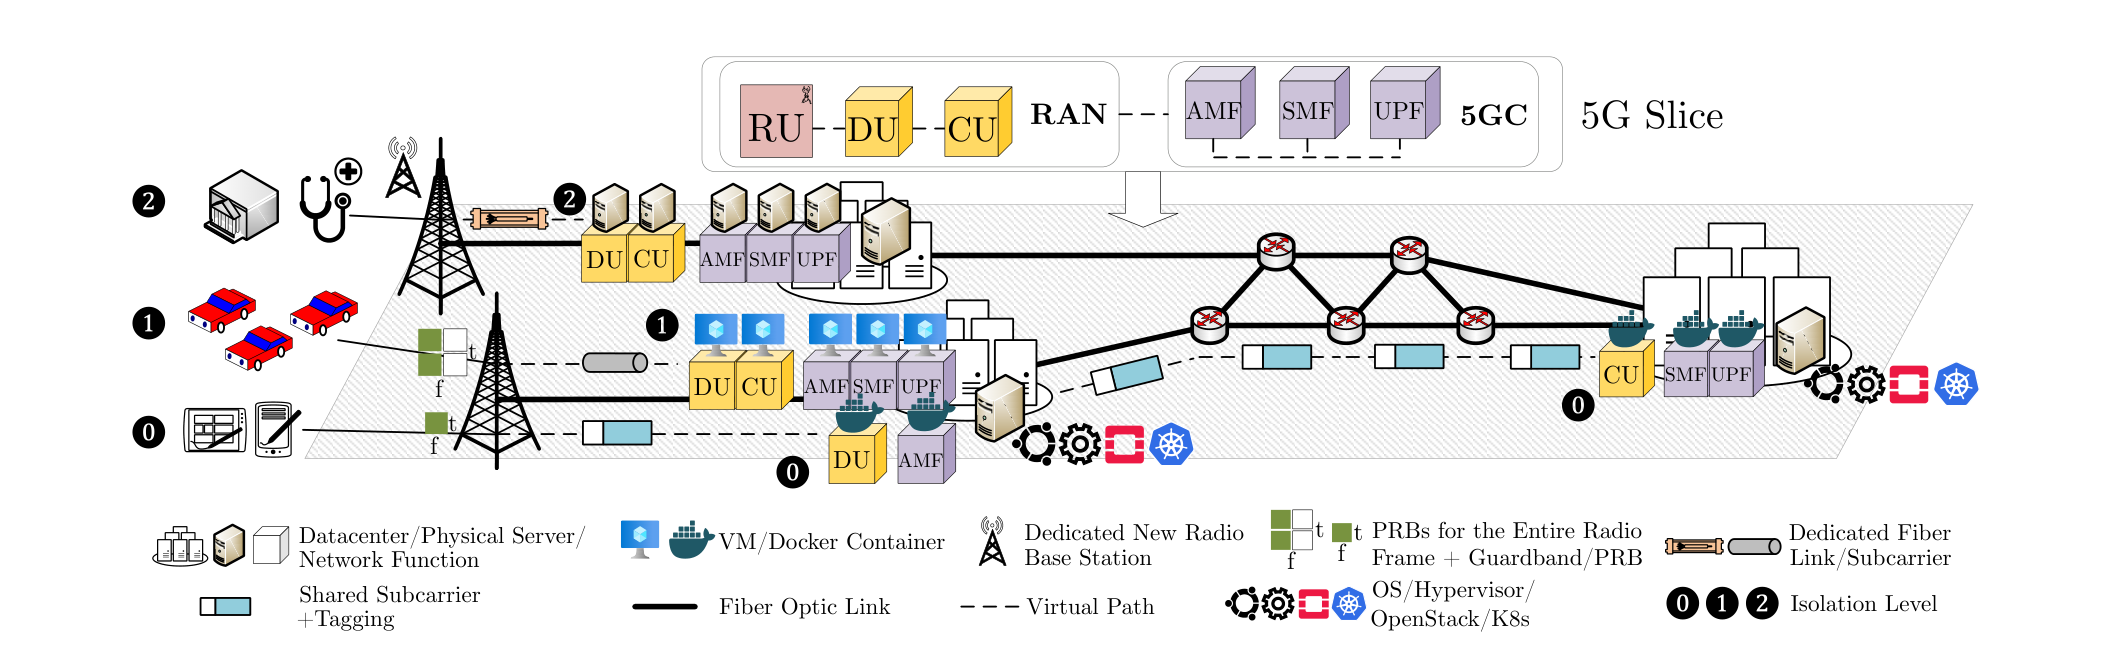
\includegraphics[width=\textwidth]{basepaper_system_model.png}
\caption[5Guard end-to-end slicing system model]{End-to-end isolation-aware 5G slicing system model. Reproduced from Fig.~1 of the 5Guard base paper~\cite{bolourian2026fiveguard}.}
\label{fig:basepaper-system-model}
\end{figure}

The three example service classes on the left of Figure~\ref{fig:basepaper-system-model} demonstrate the intended use of the levels. Critical services receive complete isolation, vehicular services receive semi-isolation, and best-effort services use shared resources. This distinction is central to SecGuard because the proposed risk engine changes the isolation input supplied to the allocator when observed traffic risk increases.

\subsection{Isolation Levels and Resource Overheads}
Figure~\ref{fig:basepaper-isolation-levels} explains how the three isolation levels are realized across the radio, transport, and MEC/cloud domains. At Level 0, slices share radio blocks, transport capacity, and containerized computing resources. Level 1 introduces stronger logical separation through radio guard bands, dedicated wavelength portions, virtual machines, hypervisors, and operating-system overhead. Level 2 reserves physical infrastructure, such as a dedicated base station, fiber resource, or physical server.

\begin{figure}[htbp]
\centering
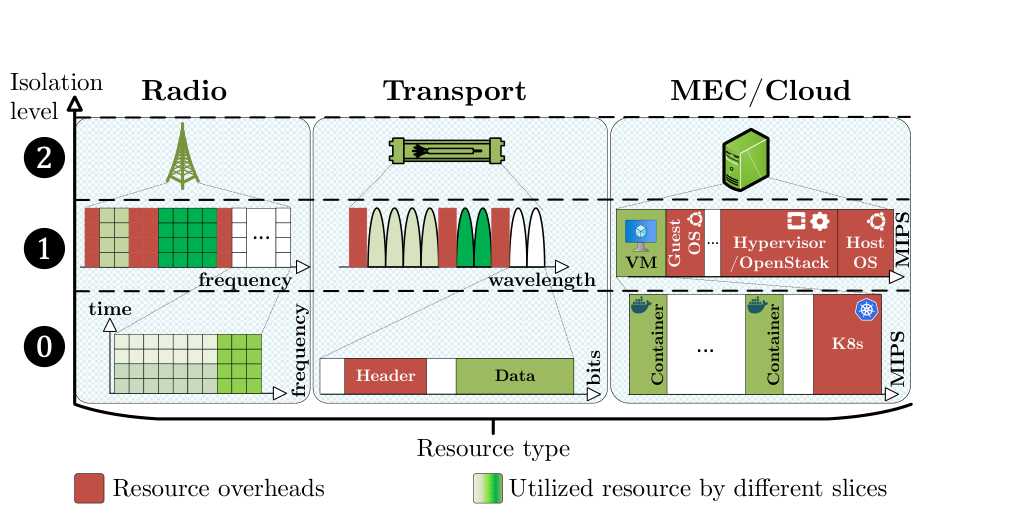
\includegraphics[width=0.72\textwidth]{basepaper_isolation_levels.png}
\caption[5Guard isolation levels and resource overheads]{Isolation levels and their resource overheads in the radio, transport, and MEC/cloud domains. Reproduced from Fig.~2 of the 5Guard base paper~\cite{bolourian2026fiveguard}.}
\label{fig:basepaper-isolation-levels}
\end{figure}

The red portions in Figure~\ref{fig:basepaper-isolation-levels} represent overhead introduced by isolation mechanisms. Stronger isolation can therefore improve separation while consuming capacity that could otherwise admit additional slices. This security--resource trade-off motivates SecGuard's use of risk-dependent upgrades instead of assigning the strongest isolation level to every slice.

Table~\ref{tab:isolation-summary} summarizes the isolation mechanisms illustrated in the base paper and the corresponding resource trade-offs.
\begin{table}[htbp]
\centering\small
\caption[Isolation mechanisms across network domains]{Isolation mechanisms across network domains, summarized from 5Guard~\cite{bolourian2026fiveguard}}
\label{tab:isolation-summary}
\renewcommand{\arraystretch}{1.2}
\begin{tabularx}{\textwidth}{|p{0.08\textwidth}|Y|Y|Y|}
\hline
\textbf{Level} & \textbf{Radio} & \textbf{Transport} & \textbf{MEC/cloud} \\
\hline
L0 & Shared base station with scheduled radio blocks & Shared subcarriers with tagging & Containerized functions on shared computing infrastructure \\
\hline
L1 & Radio blocks reserved across a frame with guard bands & Dedicated subcarriers and guard bands & Virtual machines with guest OS and hypervisor overhead \\
\hline
L2 & Dedicated base station & Dedicated fiber resource & Dedicated physical server \\
\hline
\end{tabularx}
\end{table}

\subsection{5Guard Ensemble Workflow}
Figure~\ref{fig:basepaper-flow} presents the 5Guard decision process. OPT, RNR, DTR, and IAR receive the same network state and slice request and run concurrently. Each algorithm offers a different balance between execution time and profit. When the allocation deadline is reached, unfinished executions are stopped and the framework selects the most profitable feasible solution returned within the deadline.

\begin{figure}[htbp]
\centering
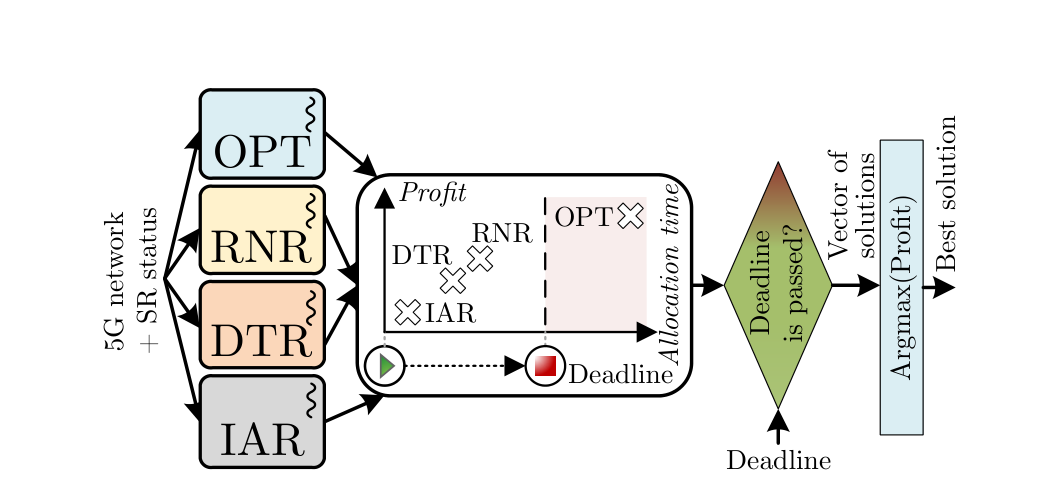
\includegraphics[width=0.68\textwidth]{basepaper_5guard_flow.png}
\caption[5Guard ensemble workflow]{Flow of the 5Guard optimization ensemble and deadline-based solution selection. Reproduced from Fig.~3 of the 5Guard base paper~\cite{bolourian2026fiveguard}.}
\label{fig:basepaper-flow}
\end{figure}

This workflow provides the allocation foundation used by SecGuard. The current contribution changes the isolation requirement presented to the allocator; it does not replace 5Guard's resource-placement formulation. The planned algorithm-selection objective would later use request and network features to avoid running unsuitable ensemble members when their expected computation cost is too high.

\section{Related Methods and Research Gap}\label{sec:gap}
The 5Guard formulation connects requested isolation levels to end-to-end resource placement, but the request is fixed at admission. SecGuard studies a separate control question: how traffic-derived risk can change the isolation input while retaining the tenant's minimum requested level. Random forests provide the classifier used for traffic risk estimation~\cite{breiman2001random}; the 5G intrusion dataset supplies the flow records used in the preliminary detector experiment~\cite{open5gsdataset}. The work reported here integrates these components with a 5Guard-style allocator. It does not establish prevention of cross-slice attack propagation.

Prior work has examined isolation-aware resource allocation and service orchestration in 5G slicing~\cite{su2019isolation,taleb2019industrial}. SecGuard builds on this line of work by connecting a traffic-derived risk signal to the isolation request passed to the allocator.

\section{Research Questions}\label{sec:research-questions}
This report asks whether a traffic-risk policy can preserve the requested isolation floor while reducing a modeled exposure measure, how much profit is recovered relative to a fixed security policy, and what remains to be tested before admission control and algorithm selection can be evaluated.


\chapter{Proposed Methodology}\label{chap:methodology}
\vspace{-1cm}
\emph{This chapter presents the design and implementation of SecGuard. Section~\ref{sec:system-design} describes the 5Guard architecture, the threat-scoring policy, and the three research objectives. Section~\ref{sec:implementation} explains the dataset, machine-learning pipeline, baseline implementation, adapter integration, and threshold-policy selection process.}
\section{System Design and Architecture}\label{sec:system-design}
\subsection{Base Architecture: The 5Guard Framework}
The foundational architecture models a 5G network across three distinct domains: Radio Access Network (RAN), Transport Network, and Edge/Core Cloud. 

\subsubsection{Isolation Levels (L0, L1, L2)}
The concept of isolation is mathematically quantified through resource overhead penalties:
\begin{itemize}
    \item \textbf{Level 0 (L0):} Shared infrastructure with containerized functions and multiplexed radio and transport resources. Computing and orchestration overhead can still be present.
    \item \textbf{Level 1 (L1):} Semi-isolation through virtual machines and reserved radio and transport portions, with hypervisor, operating-system, and guard-band overhead.
    \item \textbf{Level 2 (L2):} Complete isolation using dedicated base stations, fiber resources, and physical servers, reducing opportunities for multiplexing.
\end{itemize}

\subsubsection{MILP Optimization Objective}
The 5Guard solver seeks to maximize long-term profit $\mathcal{P}$, defined as:
\begin{equation}
    \max \mathcal{P} = \sum (\text{Revenue} - C_{dep} - C_{iso} - C_{mig} - C_{vio})
\end{equation}
Where $C_{dep}$ is deployment cost, $C_{iso}$ is the isolation overhead penalty, $C_{mig}$ is the live-migration cost of moving VNFs to satisfy constraints, and $C_{vio}$ is the SLA violation penalty if latency constraints are breached.

\subsection{Objective 1: Intelligent Security-to-Isolation Mapping}
To evolve 5Guard into SecGuard, we design a transparent security abstraction layer that intercepts slice telemetry before it reaches the 5Guard MILP solver.

\subsubsection{Threat Detection via Telemetry}
We architect an Intrusion Detection System (IDS) at the UPF (User Plane Function) that collects packet-level telemetry (e.g., flow duration, inter-arrival time, byte counts). A Machine Learning classifier (Random Forest) evaluates these flows to detect anomalous patterns indicative of DDoS, brute force, or botnet activity.

\subsubsection{Risk Aggregation and Scoring}
Packet-level predictions are mathematically aggregated into a rolling \textbf{Slice Threat Score (STS)}, normalized between $0$ and $1$. 
\begin{equation}
    STS_i = \alpha \cdot STS_{i}^{prev} + (1 - \alpha) \cdot \frac{N_{malicious}}{N_{total}}
\end{equation}
Where $\alpha$ is a temporal decay factor, smoothing the risk score over time to prevent erratic isolation oscillation.

\subsubsection{SLA-Safe Dynamic Policy Engine}
Based on the $STS_i$, the Policy Engine decides the new isolation level. A critical design constraint of SecGuard is \textbf{SLA Floor Safety}: The system may \textit{upgrade} a slice's isolation to protect the network, but it may \textit{never downgrade} it below the tenant's paid SLA. 
\begin{itemize}
    \item If $STS_i > \tau_{quarantine}$, the slice is marked for a quarantine action in the simulation.
    \item If $STS_i > \tau_{L2}$, the slice is upgraded to L2 (Physical Isolation).
    \item If $STS_i > \tau_{L1}$, the slice is upgraded to L1 (Virtual Isolation).
\end{itemize}
Choosing the exact thresholds ($\tau_{L1}, \tau_{L2}, \tau_{quarantine}$) is extremely difficult, as naive thresholds destroy profit. We address this via Surrogate ML Optimization in the implementation phase.

\subsection{Objective 2: Learning-Based Admission Control (Proposed)}
The base 5Guard uses greedy admission control; it admits any slice if current resources allow. However, admitting a large, highly isolated L2 slice now might block five highly profitable L0 slices tomorrow. We propose a Deep Q-Network (DQN) RL agent. The state space encompasses the real-time resource utilization matrices of the RAN, Transport, and Core. The action space is discrete: \{Admit, Reject, Defer\}. The reward signal is the discounted future profit derived from the 5Guard MILP.

\subsection{Objective 3: Intelligent Algorithm Selection (Proposed)}
5Guard runs ensemble members concurrently and selects the most profitable feasible solution available within the allocation deadline. We propose a lightweight Random Forest meta-classifier to select candidate algorithms using request features and network load. Its effect on execution time and solution quality remains to be evaluated.

\begin{figure}[h!]
\centering
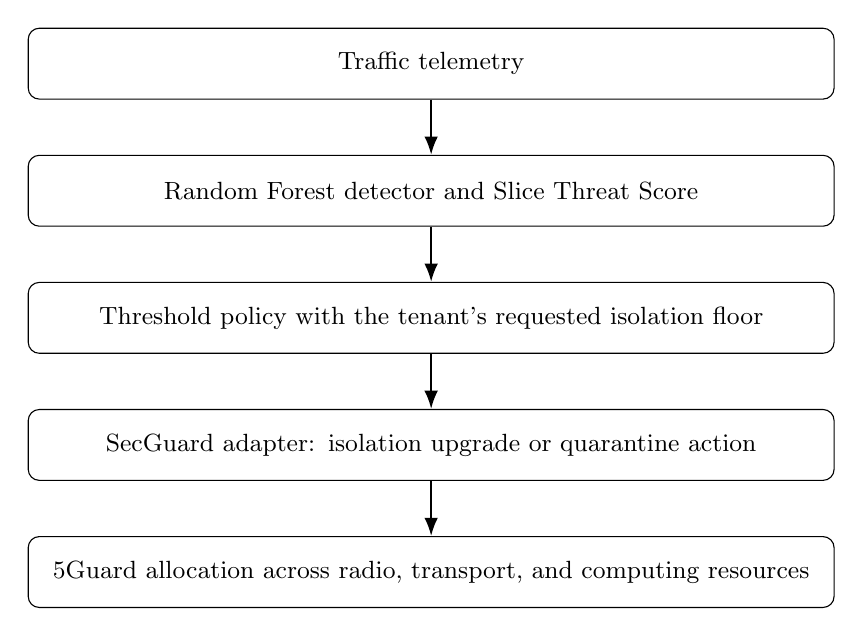
\begin{tikzpicture}[node distance=7mm,box/.style={draw,rounded corners,align=center,text width=10cm,minimum height=9mm,font=\small},flow/.style={-{Latex},thick}]
\node[box] (telemetry) {Traffic telemetry};
\node[box,below=of telemetry] (risk) {Random Forest detector and Slice Threat Score};
\node[box,below=of risk] (policy) {Threshold policy with the tenant's requested isolation floor};
\node[box,below=of policy] (adapter) {SecGuard adapter: isolation upgrade or quarantine action};
\node[box,below=of adapter] (allocation) {5Guard allocation across radio, transport, and computing resources};
\draw[flow] (telemetry)--(risk);
\draw[flow] (risk)--(policy);
\draw[flow] (policy)--(adapter);
\draw[flow] (adapter)--(allocation);
\end{tikzpicture}
\caption{Conceptual SecGuard workflow for Objective 1}
\label{fig:arch}
\end{figure}

\clearpage

\section{Implementation}\label{sec:implementation}
\subsection{Dataset and Threat Detection}
To implement Objective 1, we utilized an established 5G NIDD (Network Intrusion Detection Dataset) containing simulated 5G control plane and user plane attacks. 
The dataset consists of millions of network flows characterized by 44 statistical features.

\subsubsection{Machine Learning Pipeline}
We implemented a Random Forest Classifier using Python's \texttt{scikit-learn} library. The model was configured with 300 decision trees (\texttt{n\_estimators=300}) and a maximum depth of 20 to prevent overfitting. 
Feature engineering included normalizing continuous variables (e.g., bytes per second) and encoding categorical flags. The dataset was split 70/30 for training and testing.

\subsection{The 5Guard Baseline Implementation}
Implementing the base 5Guard paper was a significant engineering undertaking requiring the translation of theoretical mathematical models into a functional simulator. The core network environment was developed in Python, utilizing the \texttt{NetworkX} library to model the physical network substrate as a complex Multi-Graph representing interconnected RAN, Edge, and Core data centers. 

While the original paper utilized the commercial Gurobi Optimizer for its exact MILP solver (\texttt{OPT}), we were unable to secure commercial Gurobi licenses for this project. To overcome this limitation, we migrated the mathematical formulation to the open-source \textbf{SCIP} (Solving Constraint Integer Programs) optimization suite through its Python interface~\cite{gamrath2022scip}.

We defined over 50 complex linear constraints within the SCIP environment. These equations rigorously mapped VNF CPU and memory demands to physical nodes, strictly enforced link bandwidth capacities, and mathematically guaranteed isolation properties (e.g., ensuring that two VNFs belonging to different L2 slices are mutually excluded from ever sharing the same physical server). The SCIP solver proved highly capable of finding exact optimal placements, though its exponential time complexity motivated our implementation of the heuristic fallbacks. The heuristic algorithms (\texttt{IAR} and \texttt{DTR}) were implemented as custom Python classes that execute greedy, breadth-first graph-traversal algorithms to find sub-optimal but extremely fast embeddings when SCIP timed out.

\subsection{SecGuard Adapter Integration}
To seamlessly integrate Objective 1 without rewriting the entire 5Guard MILP, we implemented the \texttt{Adapter Pattern}. The \texttt{SecGuardAdapter} sits between the incoming slice requests and the 5Guard algorithms. 
For every simulation timestep, the adapter:
\begin{enumerate}
    \item Reads the current Slice Threat Score (STS) generated by the Random Forest classifier.
    \item Evaluates the policy thresholds.
    \item Constructs an adapted request with an isolation input at least as high as the tenant's requested level.
    \item Forwards the adapted request to the 5Guard allocation routine.
\end{enumerate}

Table~\ref{tab:policy-actions} summarizes the policy described in this report. The conditions are evaluated from the highest threshold downward; a quarantine action is handled separately from the three isolation levels.
\begin{table}[htbp]
\centering\small
\caption{Threat-score conditions and isolation actions}
\label{tab:policy-actions}
\renewcommand{\arraystretch}{1.2}
\begin{tabularx}{\textwidth}{|Y|Y|}
\hline
\textbf{Condition} & \textbf{Action} \\
\hline
$STS_i>\tau_{quar}$ & Request quarantine in the simulation. \\
\hline
$\tau_{L2}<STS_i\leq\tau_{quar}$ & Set isolation to L2, preserving the requested floor. \\
\hline
$\tau_{L1}<STS_i\leq\tau_{L2}$ & Set isolation to at least L1 and retain L2 if requested. \\
\hline
$STS_i\leq\tau_{L1}$ & Retain the tenant's requested isolation level. \\
\hline
\end{tabularx}
\end{table}

\subsection{Surrogate Policy Learning for Threshold Optimization}
A critical challenge in Objective 1 was defining the threshold values ($\tau_{L1}, \tau_{L2}, \tau_{quar}$) that dictate when a slice's isolation is upgraded. Hand-tuning these thresholds is impossible because the relationship between security thresholds and 5Guard's final profit is highly non-linear due to the MILP constraints.

To solve this, we used a \textbf{Surrogate ML Optimization Pipeline}:
\begin{itemize}
    \item We enumerated 165 threshold combinations in the policy search space.
    \item We evaluated candidate policies in the synthetic allocator simulation, recording profit and the modeled isolation-exposure proxy.
    \item We trained a \textit{Random Forest Regressor} surrogate model to learn the mapping from Thresholds $\rightarrow$ (Profit, Exposure).
    \item We queried the surrogate model to plot a Pareto Frontier, allowing us to select candidate thresholds that maximize profit while keeping exposure below acceptable limits.
\end{itemize}

\begin{figure}[h!]
\centering
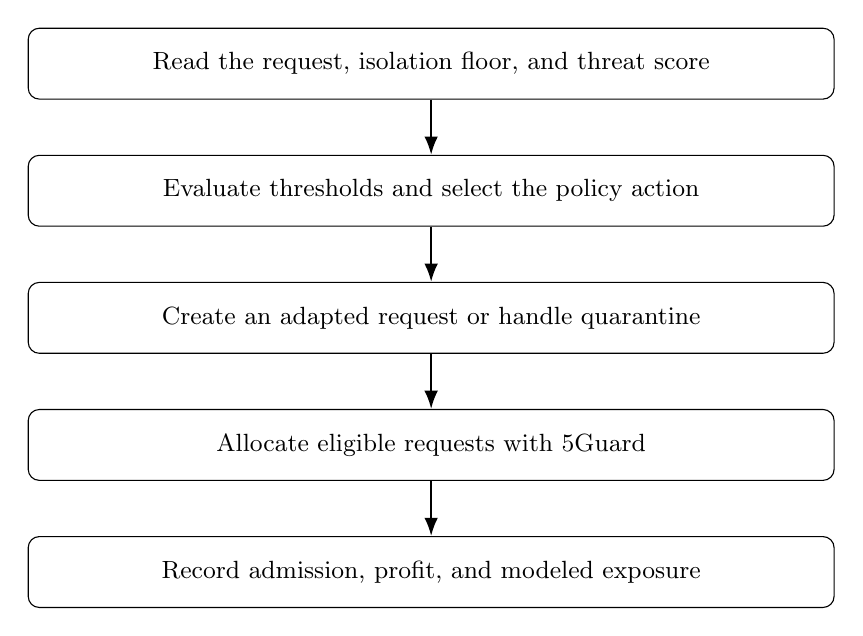
\begin{tikzpicture}[node distance=7mm,box/.style={draw,rounded corners,align=center,text width=10cm,minimum height=9mm,font=\small},flow/.style={-{Latex},thick}]
\node[box] (request) {Read the request, isolation floor, and threat score};
\node[box,below=of request] (action) {Evaluate thresholds and select the policy action};
\node[box,below=of action] (apply) {Create an adapted request or handle quarantine};
\node[box,below=of apply] (allocate) {Allocate eligible requests with 5Guard};
\node[box,below=of allocate] (record) {Record admission, profit, and modeled exposure};
\draw[flow] (request)--(action);
\draw[flow] (action)--(apply);
\draw[flow] (apply)--(allocate);
\draw[flow] (allocate)--(record);
\end{tikzpicture}
\caption{Conceptual adapter processing sequence}
\label{fig:code_impl}
\end{figure}

\clearpage


\chapter{Results and Discussion}\label{chap:results}
\vspace{-1cm}
\emph{This chapter reports and interprets the preliminary evaluation. Section~\ref{sec:evaluation-results} presents the classifier results, policy trade-off, and end-to-end comparison. Section~\ref{sec:limitations} discusses the limitations and planned extensions, and Section~\ref{sec:conclusions} summarizes the findings and the scope of the remaining work.}
\section{Results and Evaluation}\label{sec:evaluation-results}

Table~\ref{tab:evaluation-scope} summarizes the scope of the reported evaluation and distinguishes measured outcomes from proposed extensions.
\begin{table}[htbp]
\centering\small
\caption{Evaluation scope and interpretation}
\label{tab:evaluation-scope}
\renewcommand{\arraystretch}{1.2}
\begin{tabularx}{\textwidth}{|Y|Y|Y|}
\hline
\textbf{Component} & \textbf{Reported evaluation} & \textbf{Interpretation} \\
\hline
Threat detector & Within-source held-out classification & Does not establish detection of unseen attacks or networks. \\
\hline
Threshold policy & Grid of 165 candidates; selected thresholds 0.30, 0.35, and 0.90 & Selection within the modeled policy space. \\
\hline
Allocator comparison & 30 held-out trace-derived scenarios & Profit, admission, and modeled exposure in a synthetic setting. \\
\hline
Admission control and algorithm selection & Objectives 2 and 3 remain proposed & No experimental performance claim is made for these objectives. \\
\hline
\end{tabularx}
\end{table}

\subsection{Threat Classification Accuracy}
The Random Forest classifier achieved strong results on a within-source held-out test set. As shown in the confusion matrix (Figure \ref{fig:confusion}), the model achieved near 100\% accuracy, precision, and recall. This within-source test does not establish robustness to new attacks or traffic distributions; false positives can still trigger costly isolation actions.

\begin{figure}[h!]
\centering
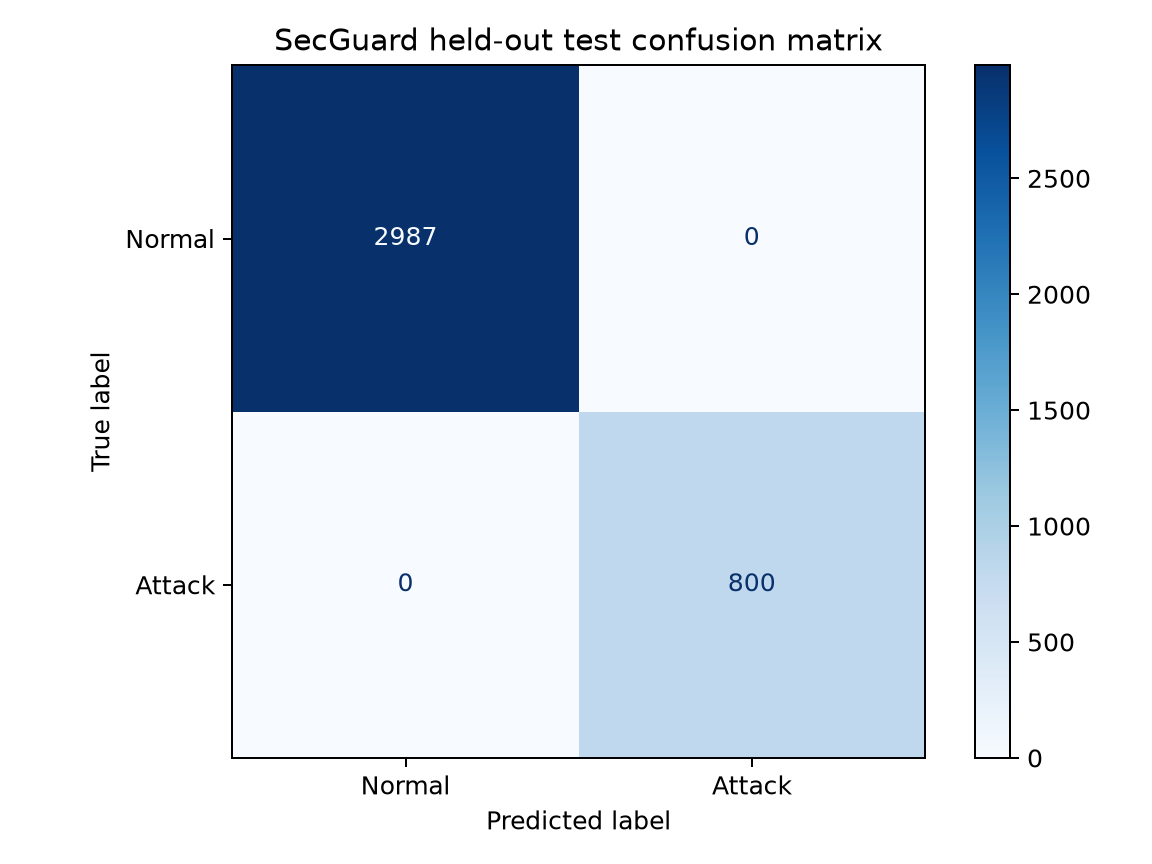
\includegraphics[width=0.6\textwidth]{confusion_matrix.png}
\caption{Confusion Matrix for Random Forest Packet Classifier}
\label{fig:confusion}
\end{figure}

\subsection{Surrogate Policy Pareto Frontier}
Figure \ref{fig:pareto} illustrates the threshold-policy trade-off over a grid of 165 candidates. The x-axis represents modeled isolation exposure (lower is better), and the y-axis represents InP profit (higher is better). The red curve shows the nondominated candidates in the plotted results.

From this frontier, the source report selected thresholds $\tau_{L1} = 0.30$, $\tau_{L2} = 0.35$, and $\tau_{quar} = 0.90$. The thresholds determine the simulated isolation action from the observed threat score.

\begin{figure}[h!]
\centering
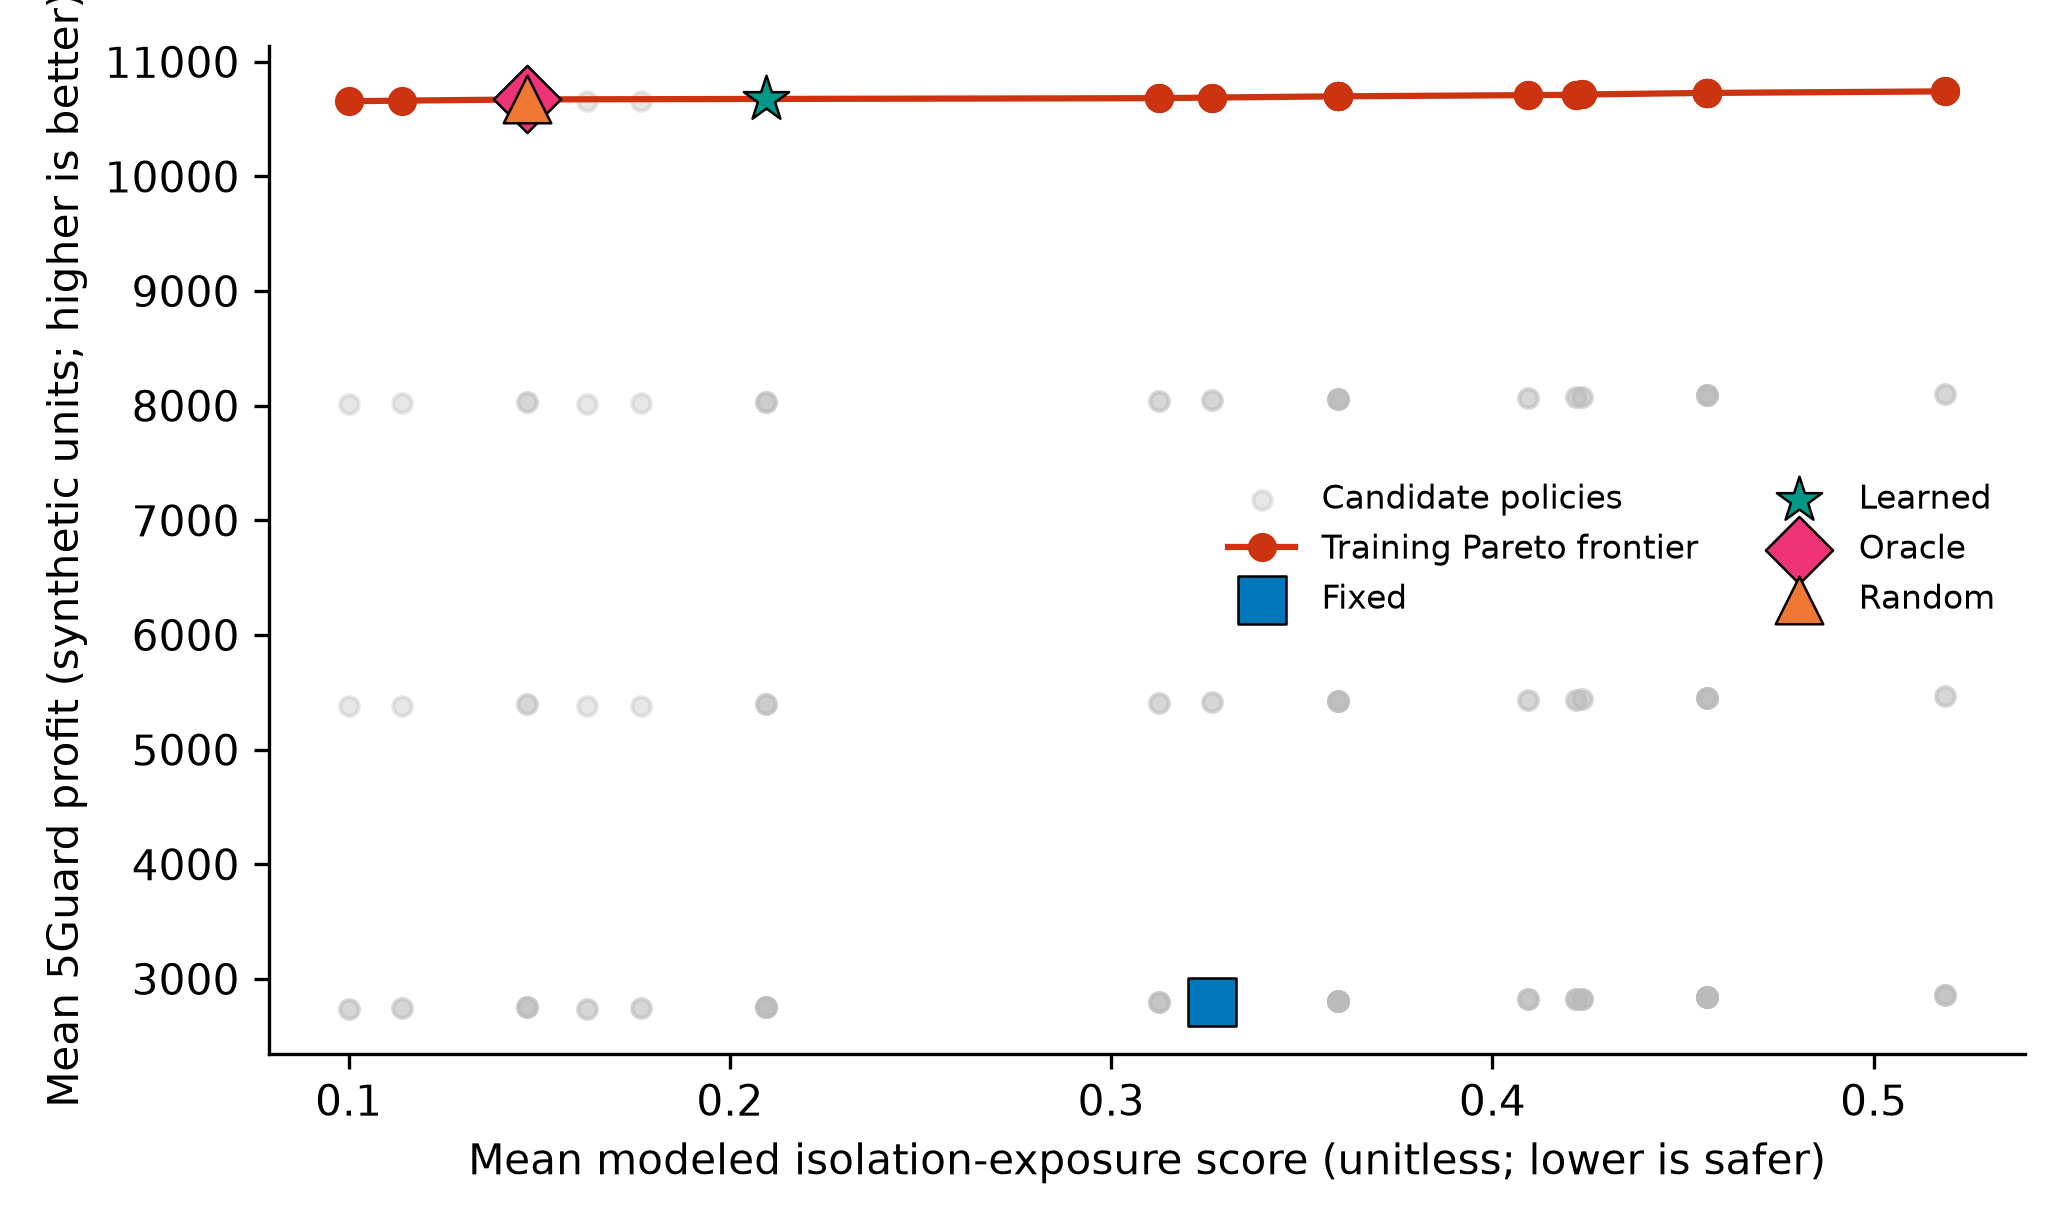
\includegraphics[width=0.7\textwidth]{pareto_frontier.png}
\caption{Pareto Frontier derived via Surrogate ML Optimization}
\label{fig:pareto}
\end{figure}

\subsection{End-to-End System Evaluation (Before vs. After)}
To rigorously validate Objective 1, we executed the 5Guard system across 30 held-out, trace-derived synthetic scenarios. We compared three distinct states:
\begin{enumerate}
    \item \textbf{Baseline 5Guard (No Security):} The original paper's logic. Isolation is purely based on static SLA requests.
    \item \textbf{Fixed SecGuard (Naive Rules):} A rigid security policy where thresholds are statically set without ML optimization.
    \item \textbf{Learned SecGuard (Our Work):} The system running our Pareto-optimal ML thresholds.
\end{enumerate}

\begin{table}[htbp]
\centering
\caption{Held-out policy results over 30 trace-derived scenarios}
\label{tab:policy-results}
\small
\begin{tabularx}{\textwidth}{Yrrrr}
\hline
\textbf{Policy} & \textbf{Mean profit} & \textbf{Exposure} & \textbf{Admitted} & \textbf{Quarantined} \\
\hline
Static 5Guard    & 8133.84 & 0.7729 & 3.00 & 0.00 \\
Fixed SecGuard   & 2776.79 & 0.2438 & 2.27 & 1.00 \\
Learned SecGuard & 7356.28 & 0.2542 & 2.90 & 0.30 \\
\hline
\end{tabularx}
\end{table}

\subsubsection{Statistical Improvements}
The preliminary comparison reports the following outcomes:
\begin{itemize}
    \item \textbf{Security Exposure Reduction:} Baseline 5Guard suffered a massive mean exposure score of 0.77. Our Learned SecGuard dropped this to 0.25, representing a \textbf{67.12\% reduction in the modeled isolation-exposure proxy}.
    \item \textbf{Profit Recovery:} The Fixed SecGuard (naive rules) over-reacted to threats, resulting in massive L2 over-provisioning and quarantines, plunging the mean profit to 2,776.7. Our Learned SecGuard intelligently balanced the risk, achieving a mean profit of 7,356.2, representing a \textbf{164.9\% higher mean profit relative to the fixed policy}.
    \item \textbf{Profit Retention:} The selected policy retained \textbf{90.4\%} of the static baseline mean profit in this evaluation.
    \item \textbf{Admission Rate:} The Learned policy admitted an average of 2.9 out of 4 slices per scenario, compared to only 2.2 for the naive policy, indicating higher admission in these scenarios.
\end{itemize}

\begin{figure}[h!]
\centering
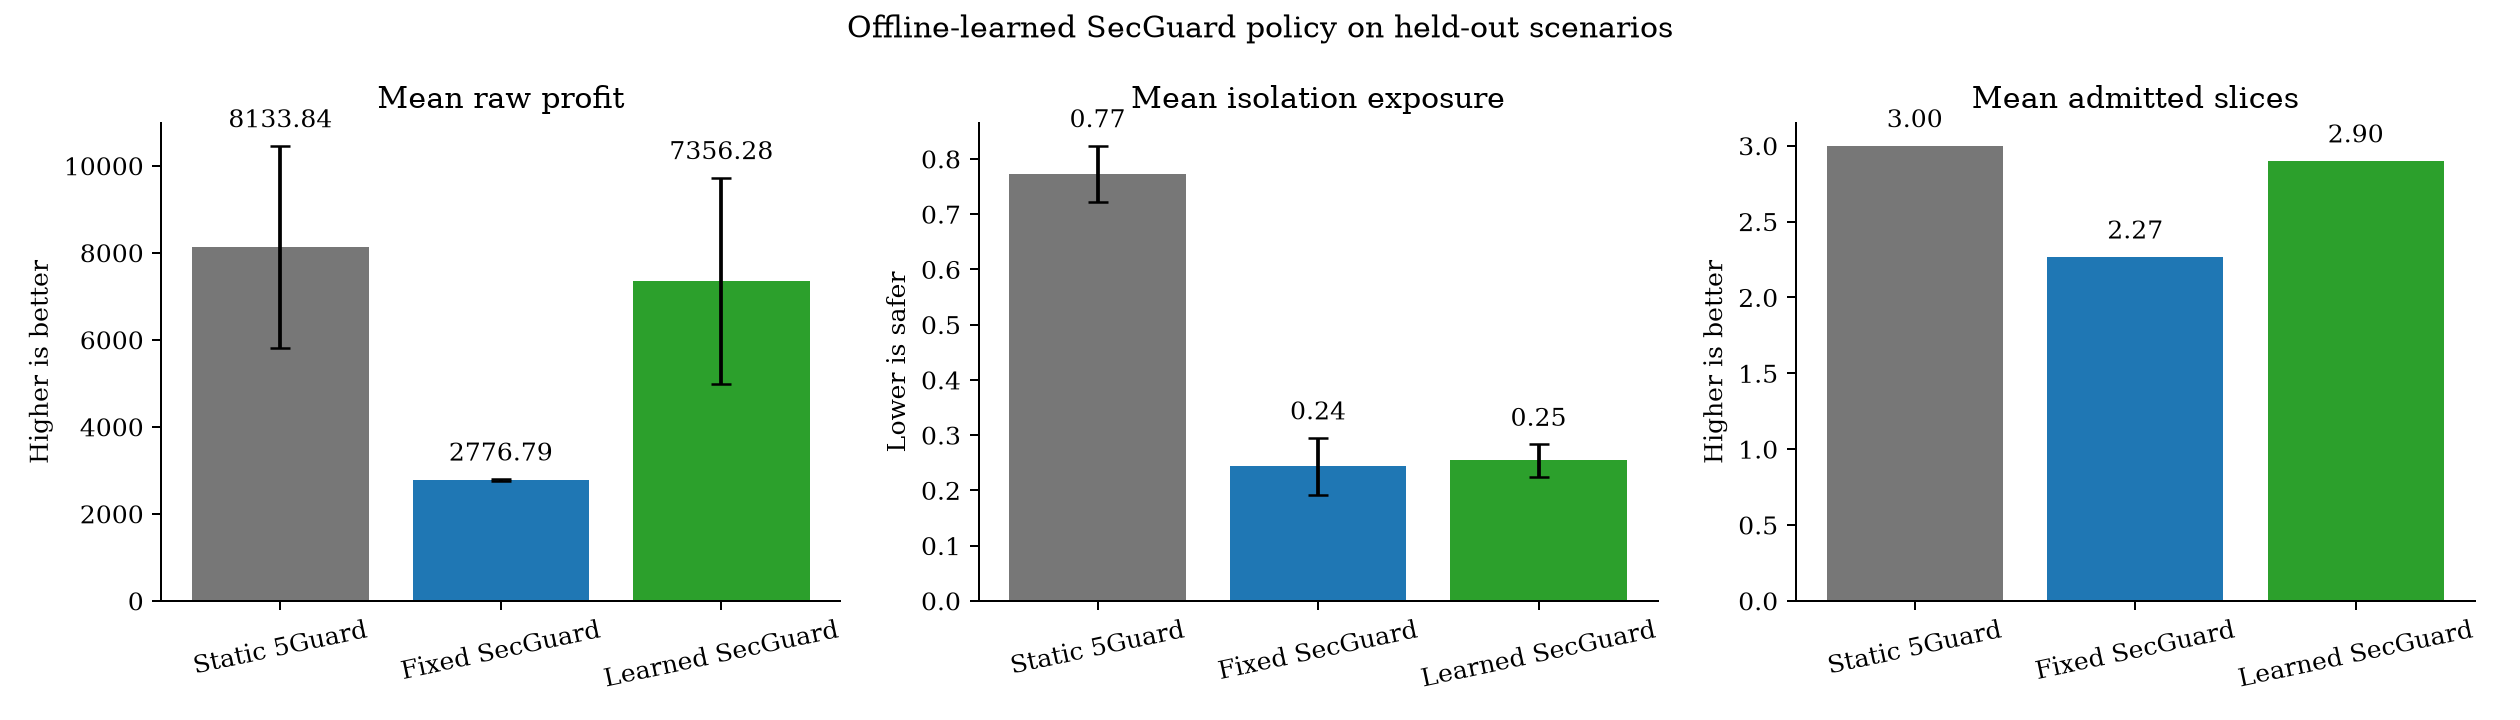
\includegraphics[width=0.7\textwidth]{learned_policy_comparison.png}
\caption{Comparison of Profit vs Security Exposure across Policies}
\label{fig:comparison}
\end{figure}

\subsection{The Security-Resource Efficiency (SRE) Metric}
For future evaluation, the source report proposes a \textbf{Security-Resource Efficiency (SRE)} measure. 
\begin{equation}
    SRE = \frac{\Delta \text{Exposure Reduction}}{\Delta \text{Isolation Overhead}}
\end{equation}
SRE requires a consistent isolation-overhead definition and should be evaluated separately before drawing an optimization claim.

\clearpage
\section{Limitations and Future Work}\label{sec:limitations}

While Objective 1 of SecGuard shows promising preliminary results, several limitations must be acknowledged:

\subsection{Adversarial Machine Learning}
The Random Forest classifier relies on standard telemetry features. Advanced attackers could utilize Adversarial ML techniques to artificially alter packet flow timings and payload sizes, effectively hiding malicious traffic below the classifier's decision boundary. Future work must incorporate robust, adversarial-aware training protocols.

\subsection{Generalization to Complex Topologies}
The MILP and heuristic simulations were executed on a medium-scale topology consisting of interconnected Edge and Core nodes. Scaling the exact MILP solver to nation-wide topologies (thousands of nodes) remains computationally intractable. This highlights the urgent necessity of \textbf{Objective 3 (Intelligent Algorithm Selection)} to intelligently route requests away from the exact solver when the graph size crosses critical complexity thresholds.

\subsection{Reinforcement Learning Stability (Objective 2)}
The proposed Deep Q-Network for Admission Control (Objective 2) faces significant challenges regarding training stability. The 5G network state space is highly stochastic and non-stationary. Future iterations of this work will explore Proximal Policy Optimization (PPO) and Multi-Agent RL to stabilize convergence.

\section{Conclusions}\label{sec:conclusions}
The preliminary evaluation reports a 67.12\% reduction in the modeled isolation-exposure proxy while retaining 90.4\% of the static baseline mean profit. These results support further investigation of risk-adaptive isolation. They do not yet establish attack containment or performance on a deployed network.

Objectives 2 and 3 remain future work. They require dedicated training and held-out evaluation before claims about admission quality or allocation latency can be made.


\fancyhead[LE]{\bfseries\small{Bibliography}}
\fancyhead[RO]{\bfseries\small{Bibliography}}
\pdfbookmark[1]{Bibliography}{bibliography}
\addstarredchapter{Bibliography}
\baselineskip 14pt
\small
\bibliographystyle{unsrt}
\bibliography{chapters/references/references}
\end{document}
